\documentclass[12pt]{article}
%%%%%%%%%%%%%%%%%%%%%%%%%%%%%%%%%%%%%%%%%%%%%%%%%%%%%%%%%%%%%%%%%%%%%%%%%%%%%%%%%%%%%%%%%%%%%%%%%%%%%%%%%%%%%%%%%%%%%%%%%%%%%%%%%%%%%%%%%%%%%%%%%%%%%%%%%%%%%%%%%%%%%%%%%%%%%%%%%%%%%%%%%%%%%%%%%%%%%%%%%%%%%%%%%%%%%%%%%%%%%%%%%%%%%%%%%%%%%%%%%%%%%%%%%%%%
\usepackage{amsfonts}
\usepackage{eurosym}
\usepackage{geometry}
\usepackage{amsmath,amsthm,amssymb}
\usepackage{ulem} 
\usepackage{graphicx}
\usepackage{comment}
%\usepackage[sort,comma]{natbib}
\usepackage[backend=biber, style = apa]{biblatex}
\usepackage{placeins} % to separate sections

\usepackage{adjustbox}
\usepackage{array}
\usepackage{multirow}
\usepackage{graphicx}
\usepackage{subcaption}
\usepackage{pifont}
\usepackage{amssymb}
\usepackage{comment}
\usepackage[utf8]{inputenc}
\usepackage{setspace}
\usepackage[hang, flushmargin, bottom]{footmisc}
\usepackage{footnotebackref}
\usepackage{xcolor}
\usepackage{hyperref}
\usepackage{booktabs}
\usepackage{pifont}
\usepackage{caption}
\usepackage{float}
\usepackage{todonotes}
\setcounter{MaxMatrixCols}{10}
%TCIDATA{OutputFilter=LATEX.DLL}
%TCIDATA{Version=5.50.0.2960}
%TCIDATA{<META NAME="SaveForMode" CONTENT="1">}
%TCIDATA{BibliographyScheme=BibTeX}
%TCIDATA{LastRevised=Sunday, April 28, 2024 18:12:38}
%TCIDATA{<META NAME="GraphicsSave" CONTENT="32">}
%TCIDATA{Language=American English}

%\setlength{\bibsep}{0.3pt}
\setlength{\textfloatsep}{5pt}
\hypersetup{breaklinks=true,hypertexnames=false,colorlinks=true,citecolor = teal}
\captionsetup{font=normalsize}
\newcommand{\cmark}{\ding{51}}
\def\sym#1{\ifmmode^{#1}\else\(^{#1}\)\fi}
\renewcommand{\thetable}{\Roman{table}}
\geometry{verbose,tmargin=.9in,bmargin=1in,lmargin=.8in,rmargin=.8in,nomarginpar}
\makeatletter
\DeclareTextSymbolDefault{\textquotedbl}{T1}
\theoremstyle{plain}
\newtheorem{thm}{\protect\theoremname}
\theoremstyle{plain}
\newtheorem{prop}[thm]{\protect\propositionname}
\providecommand{\propositionname}{Proposition}
\providecommand{\theoremname}{Theorem}
\makeatother
\providecommand{\propositionname}{Proposition}
\providecommand{\theoremname}{Theorem}
\newtheorem{ass}[thm]{Assumption}
% \input{tcilatex}
\usepackage{tikz}
\usetikzlibrary{shapes.geometric, arrows, positioning}





\addbibresource{references.bib}
\begin{document}


\textbf{Overview}

\begin{itemize}
    \item We present a model of asymmetric competition in insurance markets 
    \item We show that there is selection into the market (buyers tend to be healthier than non-buyers), but not across firms (the health distribution is the same for different firms). 
    \item Given that there is no selection across firms the average cost is the same for all firms. Despite equal average costs, firms have different marginal costs. 
\end{itemize}


\hline

\medskip

This document aims to study the impact of selection in a model of an annuities market, where buyers have private information about their health status and insurers are differentiated. 
In section \ref{sec:model} we present the demand, the insurer costs and we solve for the equilibrium. In section \ref{sec:simulation} using simulations we study the impact of a change in private information in the equilibrium outcomes. 




%In section \ref{sec:consumer_choice} we present the demand, in section \ref{sec:costs} we present the costs of the insurers, in section \ref{sec:pricing} we solve for the optimal firm prices. 

\section{The model}\label{sec:model}
\subsection{Consumer choice}\label{sec:consumer_choice}

Consider a nested logit where the outer nest consists on a choice of buying an annuity or the outside option. The inner nests consists on the choice of insurer from which to purchase. 

Denote by $\delta_j$ the mean utility of each option, where $j =0$ represents the outside option. 

Define $h_i$ the health status of buyer $i$, which is private information. Given that $h_i$ affects the expected number of payments when buying the annuity the mean utility of the insurers will depend on it, $\delta_j(h_i)$, where we assume that the mean utility is increasing on the health information. 

Assume that, for any $j\neq 0$,  $\delta_j = f(h_i) + \tilde{\delta}_j$, with $f(\cdot)$ being strictly increasing,  but health status does not affect the outside option. 


Then, the probability of choosing $j$ given conditional on buying an annuity is: 
\begin{equation}\label{eq:no_selection}
    s_{j\mid A}(h_i) = \frac{\exp((f(h_i) + \tilde{\delta}_j) / \rho)}{\sum_{k=1}^{J} \exp((f(h_i) + \tilde{\delta}_j)/ \rho)} = \frac{\exp( \tilde{\delta}_j / \rho)}{\sum_{k=1}^{J} \exp( \tilde{\delta}_j/ \rho)} \equiv s_{j\mid A}
\end{equation}
implying that, conditional on buying an annuity the health information does not affect the insurer choice. 
 

And the probability of buying an annuity is: 
\begin{align}\label{eq:into_selection}
    s_A(h_i)
    %= \frac{\alpha_A\left(\sum_{j=1}^J \exp((f(h_i) + \tilde{\delta}_j)/\rho)\right)^\rho }{\alpha_A\left(\sum_{j=1}^J \exp((f(h_i) + \tilde{\delta}_j)/\rho)\right)^\rho +  \exp \left(\delta_0 \right)} \\
    = \frac{\alpha_A\exp(f(h_i)/\delta)^\rho\left(\sum_{j=1}^J \exp(\tilde{\delta}_j/\rho)\right)^\rho }{\alpha_A\exp(f(h_i)/\delta)^\rho\left(\sum_{j=1}^J \exp(\tilde{\delta}_j/\rho)\right)^\rho  +  \exp \left(\delta_0 \right)}
\end{align}
implying that the probability of buying an annuity is increasing on health status. 


\subsection{Average and marginal costs}\label{sec:costs}

Define $c_j(h_i)$ the cost for insurer $j$ of selling an annuity to buyer with health status $h_i$, where the cost is increasing on its argument.  Then the average cost of insurer $j$ is\footnote{Remember that we are studying a particular group of the population, hence is the average cost for individuals who have the same observables. }: 

\begin{align}\label{eq:avg_cost}
    \bar{c}_j = \frac{\int c_j(h)\cdot s_j(h) \cdot f_h(h) dh}{\int  s_j(h) \cdot f_h(h) dh}
\end{align}
where $f_h(\cdot)$ is the density of health status. 

The marginal cost is: 
\begin{align}\label{eq:mg_cost}
    c^m_j = \frac{\int c_j(h) \frac{\partial s_j(h)}{\partial p_j}  f_h(h) dh }{\int \frac{\partial s_j(h)}{\partial p_j}  f_h(h) dh }
\end{align}

To obtain a closed form solution for the semi-elasticities we assume  $\tilde{\delta}_j = \hat{\delta}_j - \alpha p_j$. Then: 

\begin{align}\label{eq:price_der}
    \frac{\partial s_j(h)}{\partial p_j} 
    %= -\alpha \ s_j \left[ \left(\frac{1}{\rho}(1-s_{j|A})\right)  + s_{j|A}  (1-s_A) \right]  
    = -\alpha \ s_A(h) s_{j\mid A}(h) \left[ \left(\frac{1}{\rho}(1-s_{j|A}(h))\right)  + s_{j|A}(h)  (1-s_A(h)) \right]  
\end{align}



Note that $\frac{1}{\rho}(1-s_{j|A}(h))$ represents the consumers that are substituting from other firms and $s_{j|A}(h)  (1-s_A(h))$ represents the consumers that are substituting from the outside option. 
If the shocks within the nest are correlated ( $\rho \rightarrow 0 $) then most of the marginal consumers are susbstituting from other firms, whereas if the outside option is very relevant $s_A \rightarrow 1 $ then most of the additional consumers come from the outside option. 


Given that the  probability of buying an annuity is increasing on $h_i$ (see equation \ref{eq:into_selection}), there is adverse selection into the annuities market. The cost of selling an annuity to an annuities buyer is on average higher than the cost of providing an annuity to a buyer choosing the outside option.

If all firms have the same cost function ($c_j(h) = c(h)$), then the average cost is the same for all firms. We refer by this result as \textit{no selection across firms} since all the cost differences would arise due to different cost functions and not due to consumers sorting into firms. 

Moreover given that the non-buyers tend to be healthier than the buyers, the marginal cost is lower than the average costs. The intuition is that the marginal cost of a firm is the convex combination of the cost of buyers diverted from other firms and the cost of  buyers diverted from the outside option (see equation \ref{eq:price_der}), where this latter group has a lower cost, whereas the average cost is the same as the cost of buyers diverted from other firms.  


Even in the case firms have the same cost function, product differentiation generates  heterogeneity in marginal costs. This can appear counterintuitive, because previously we determined that there is no selection across firms which implies that they have the same average costs. To build some intuition, consider a duopoly with market shares 50\%, 1\% and 49\% does not buy the insurance. The market leader, when decreasing the costs, gets the healthy non buyers, whereas the small firms gets a mixture of previous buyers and non-buyers. Hence the bigger firm has smaller marginal costs than the smaller firm. 


\subsection{Firm pricing}\label{sec:pricing}
The firm profits are:

\begin{align}
    \pi_j &= \int ( p_j -c(h) )s_j(h) f(h) dh  
\end{align}

Using equation \ref{eq:price_der}, and defining the competition weight: 

\begin{align}\label{eq:comp_weight}
    w(h) \equiv s_A(h)s_{j|A}(h)\left[\frac{1}{\rho}(1-s_{j|A}(h)) + s_{j|A}(h)(1-s_A(h))\right]   = -\frac{1}{\alpha} \frac{\partial s_j(h)}{\partial p_j} 
\end{align}
We can write the FOC as: 
\begin{align}
    p_j- c^m_j  = \frac{ s_j}{\alpha \int w(h) f(h) dh} = 
\end{align}

and the outside share: 
\begin{align}\label{eq:outside_share2}
    s_0 = \int \left[ \frac{1}{\alpha_A e^{f(h) -\delta_0}\left[\sum_{j=1}^{J}e^{(\hat{\delta}_j  - \alpha p_j)/\rho}\right]^\rho + 1 } \right] f_h(h) dh
\end{align}


\subsection{Effect of increasing information}

In the model we presented, $h_i$ is the private information of the buyer. Providing more information to the sellers implies reducing the role of private information, which we interpret as a decrease in the variance of $h_i$. Assuming that $h_i$ is normally distributed with mean $0$ and standard deviation $\sigma$, we can use our previous results to study the impact of information in various outcomes.

\begin{itemize}
    \item From equation \ref{eq:outside_share2} we can calculate the market share of the outside product and determine what happens when we reduce the role of private information. 

    \item From equations \ref{eq:avg_cost} and \ref{eq:mg_cost} we can calculate the average cost and the marginal cost as a function of $\sigma$ and from them determine the degree of adverse selection. 

\end{itemize}


Note that given that we do not have a close form solution for the equilibrium prices, and as a consequence neither for the market shares and costs, we will perform simulations. In the next section we present the functional forms used and the results obtained. 




\section{Simulation}\label{sec:simulation}

For the simulations we assume that the cost function of the firm is the same for all of them and is given by: 
$c(h) = c_0 + \gamma \cdot h$

Figure \ref{fig:1} shows i) the average cost is higher than the marginal cost and ii) the marginal costs are not the same across firms. This could appear to be counterintuitive given in equation \ref{eq:no_selection} we proved that the distribution of consumers for the different firms is the same, but hinges on the fact that the diversion ratio from the outside option for the different firms is different. A third pattern of the figure is that average and marginal costs increase when the amount of private information increases. 



\begin{figure}[H]
\caption{}
 \label{fig:1}
\centering{}%
\begin{tabular}{cc}
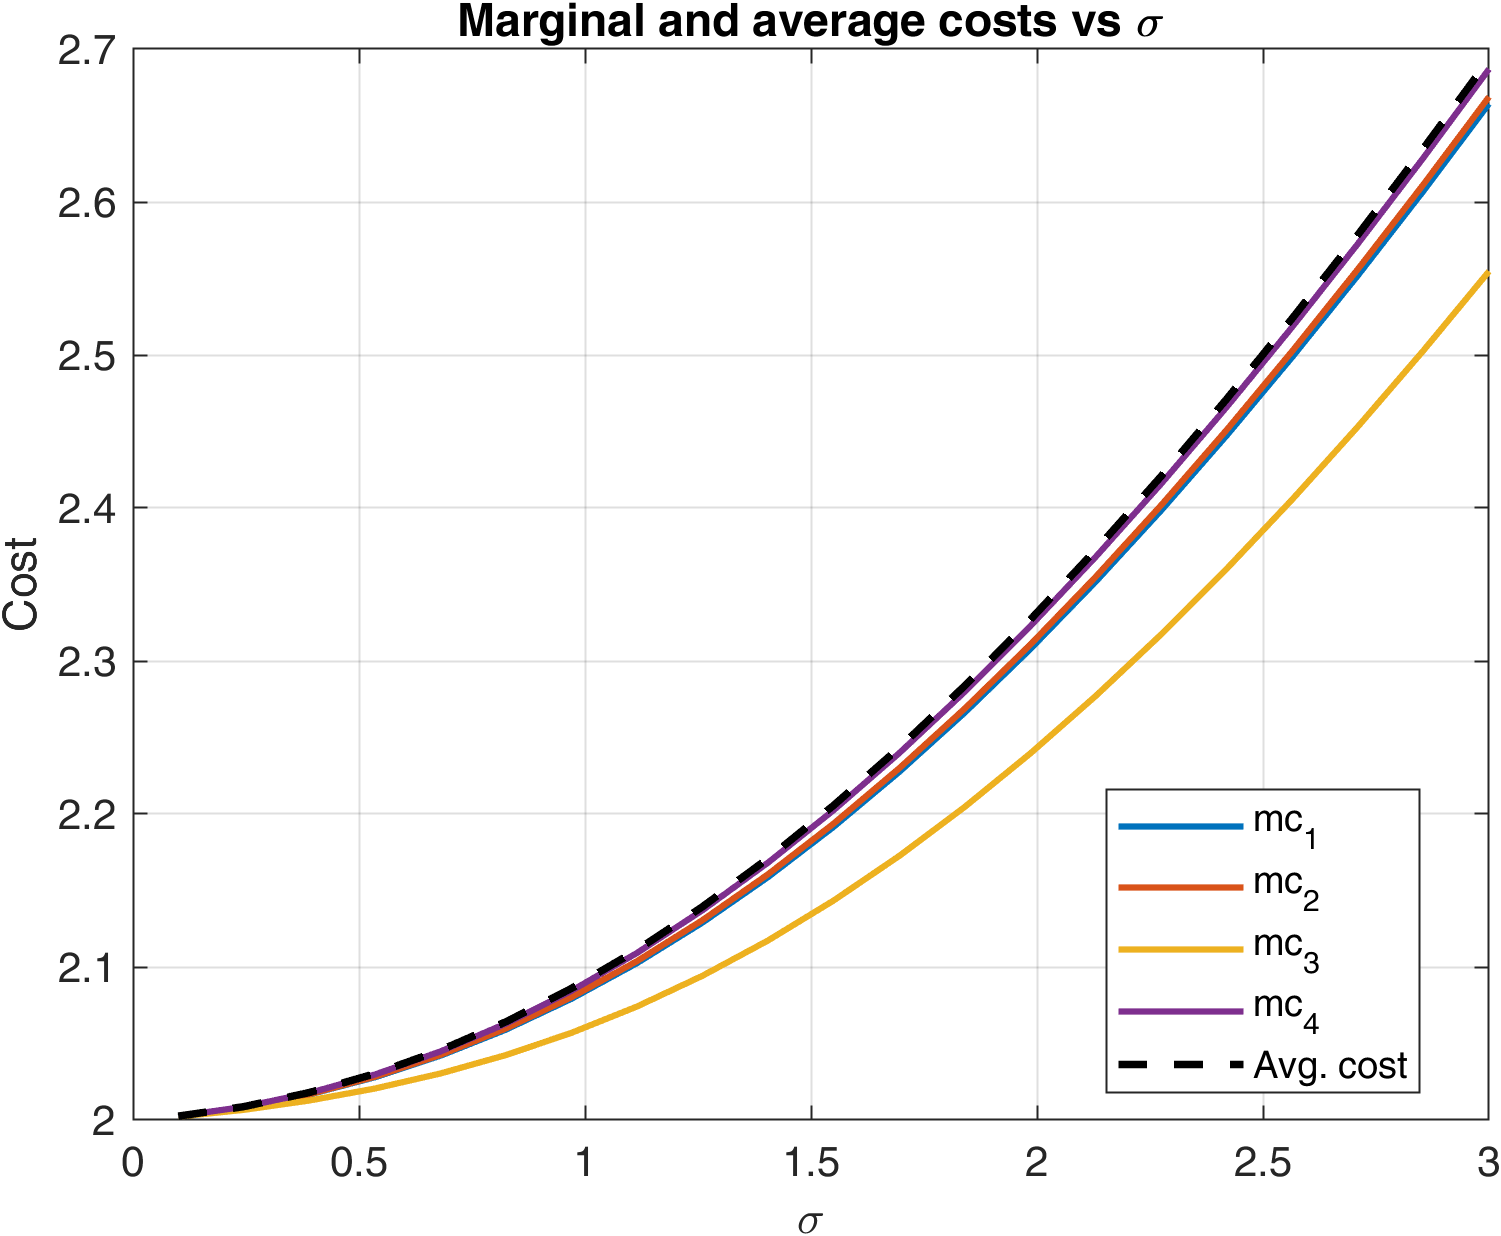
\includegraphics[scale=0.61]{figures/simulations/costs_vs_sigma.png} 
\end{tabular}
\end{figure}
Figure \ref{fig:2} left panel shows the market shares as function of $\sigma$. The main pattern is that when the amount of private information increases (higher $\sigma$) there is unraveling, the amount of individuals choosing the outside option grows. This is generated by higher prices (right panel) which are driven by an increase of prices. 


\begin{figure}[H]
\caption{}
 \label{fig:2}
\centering{}%
\begin{tabular}{cc}
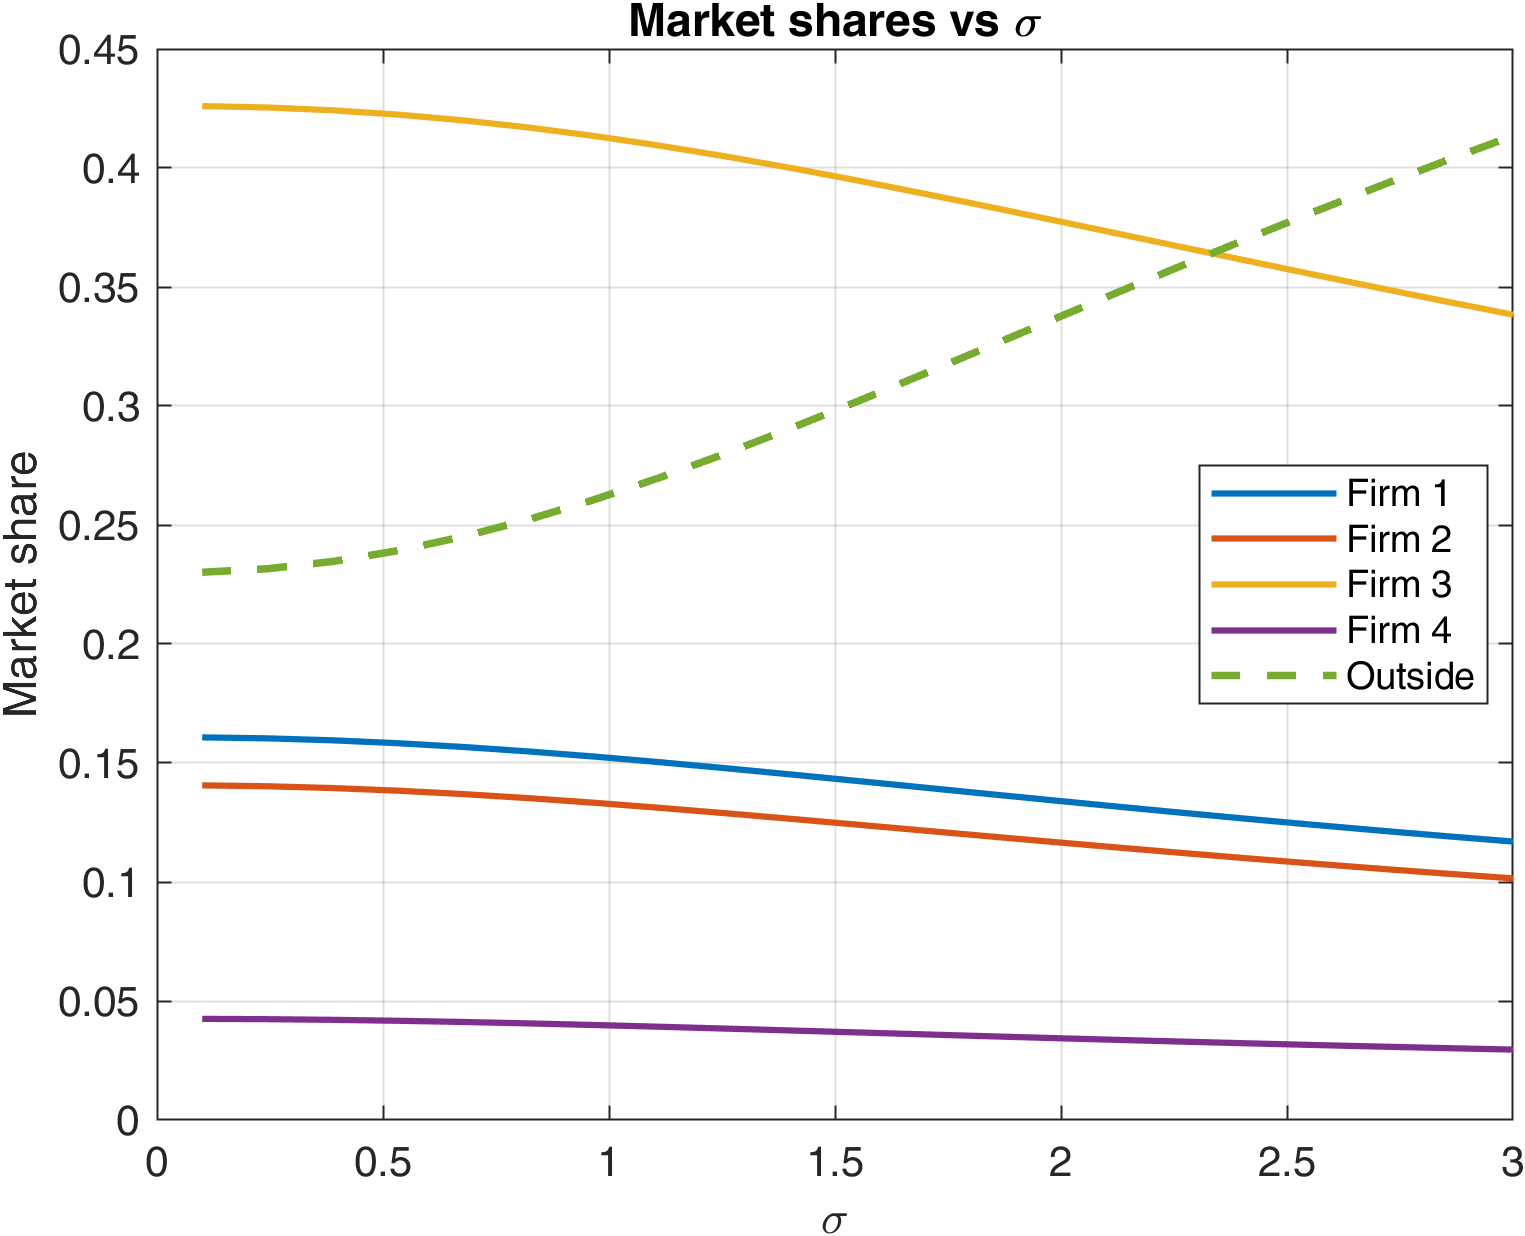
\includegraphics[scale=0.61]{figures/simulations/shares_vs_sigma.png} & 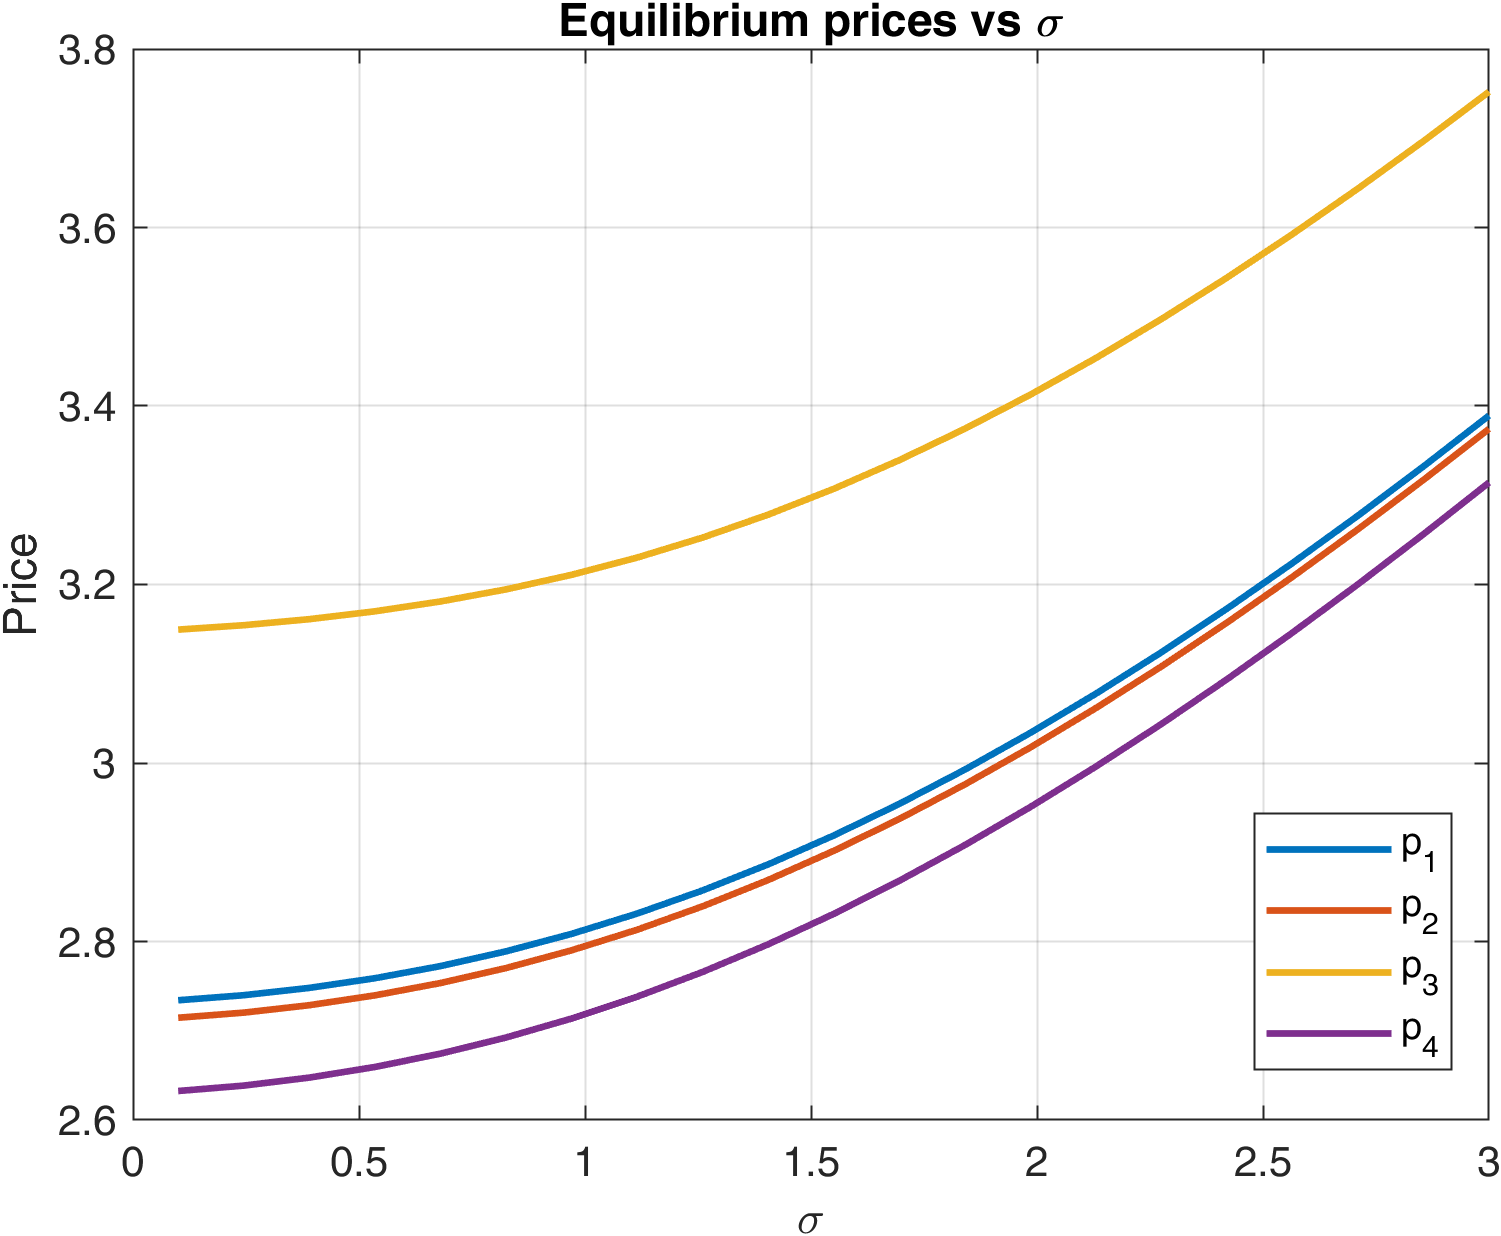
\includegraphics[scale=0.61]{figures/simulations/prices_vs_sigma.png}
\end{tabular}
\end{figure}
\newpage
  

 
\end{document}